\documentclass[11pt,onside]{article}
\usepackage[a4paper,left=3cm,right=3cm,top=2.5cm,bottom=2.5cm]{geometry}
\usepackage[utf8]{inputenc}
\usepackage[english]{babel}
\usepackage{lipsum}
\usepackage{bm}
\usepackage{upgreek}
\usepackage{booktabs}
\usepackage{graphicx}

\usepackage{amsmath}
% mathtools for: Aboxed (put box on last equation in align envirenment)
\usepackage{microtype} %improves the spacing between words and letters

%% COLOR DEFINITIONS

\usepackage[svgnames]{xcolor} % Enabling mixing colors and color's call by 'svgnames'

\definecolor{MyColor1}{rgb}{0.2,0.4,0.6} %mix personal color
\newcommand{\textb}{\color{Black} \usefont{OT1}{lmss}{m}{n}}
\newcommand{\blue}{\color{MyColor1} \usefont{OT1}{lmss}{m}{n}}
\newcommand{\blueb}{\color{MyColor1} \usefont{OT1}{lmss}{b}{n}}
\newcommand{\red}{\color{LightCoral} \usefont{OT1}{lmss}{m}{n}}
\newcommand{\green}{\color{Turquoise} \usefont{OT1}{lmss}{m}{n}}

\DeclareMathOperator{\trace}{trace}
\DeclareMathOperator{\diag}{diag}

%% FONTS AND COLORS

%    SECTIONS

\usepackage{titlesec}
\usepackage{sectsty}
%%%%%%%%%%%%%%%%%%%%%%%%
%set section/subsections HEADINGS font and color
\sectionfont{\color{MyColor1}}  % sets colour of sections
\subsectionfont{\color{MyColor1}}  % sets colour of sections

%set section enumerator to arabic number (see footnotes markings alternatives)
\renewcommand\thesection{\arabic{section}.} %define sections numbering
\renewcommand\thesubsection{\thesection\arabic{subsection}} %subsec.num.

%define new section style
\newcommand{\mysection}{
\titleformat{\section} [runin] {\usefont{OT1}{lmss}{b}{n}\color{MyColor1}} 
{\thesection} {3pt} {} } 


%	CAPTIONS
%\usepackage{caption}
%\usepackage{subcaption}
%%%%%%%%%%%%%%%%%%%%%%%%
%\captionsetup[figure]{labelfont={color=Turquoise}}


%		!!!EQUATION (ARRAY) --> USING ALIGN INSTEAD
%using amsmath package to redefine eq. numeration (1.1, 1.2, ...) 
\renewcommand{\theequation}{\thesection\arabic{equation}}



\makeatletter
\let\reftagform@=\tagform@
\def\tagform@#1{\maketag@@@{(\ignorespaces\textcolor{red}{#1}\unskip\@@italiccorr)}}
\renewcommand{\eqref}[1]{\textup{\reftagform@{\ref{#1}}}}
\makeatother
\usepackage{hyperref}
\hypersetup{colorlinks=true}

% For labeling top of page on every page but first one:
\usepackage{fancyhdr}

% PREPARE TITLE:
\title{\blue Optimization \\
\blueb Homework 1}
\author{Hector G. Flores Rodriguez (Id. 25721714)}
\date{\today} % You can set the date automatically by replacing "date goes here" with "\today"

\renewcommand{\rmdefault}{phv} % Arial Font
\renewcommand{\sfdefault}{phv} % Arial Font

\pagestyle{fancy}
\fancyhead{}
\fancyhead[CO,CE]{{\small{{\bf{Homework 1}} - Optimization - Fall 2017 - Hector G. Flores}}}
 


\begin{document}
\maketitle

\section{Problem 1}
\begin{description}
\item[1-(b)] The Fibonnacci method was used to optimized the functions:

\begin{align*}
f_{1}(x) &= x^2 + 2x \\
f_{2}(x) &= x^3 - 13x^2 + 36
\end{align*}

Prior to optmizing the provided functions, an initial interval for candidate starting points was determined by visually inspecting the graphs of the functions (shown in Figure~\ref{fig:functions}). 

\begin{figure}[h]
  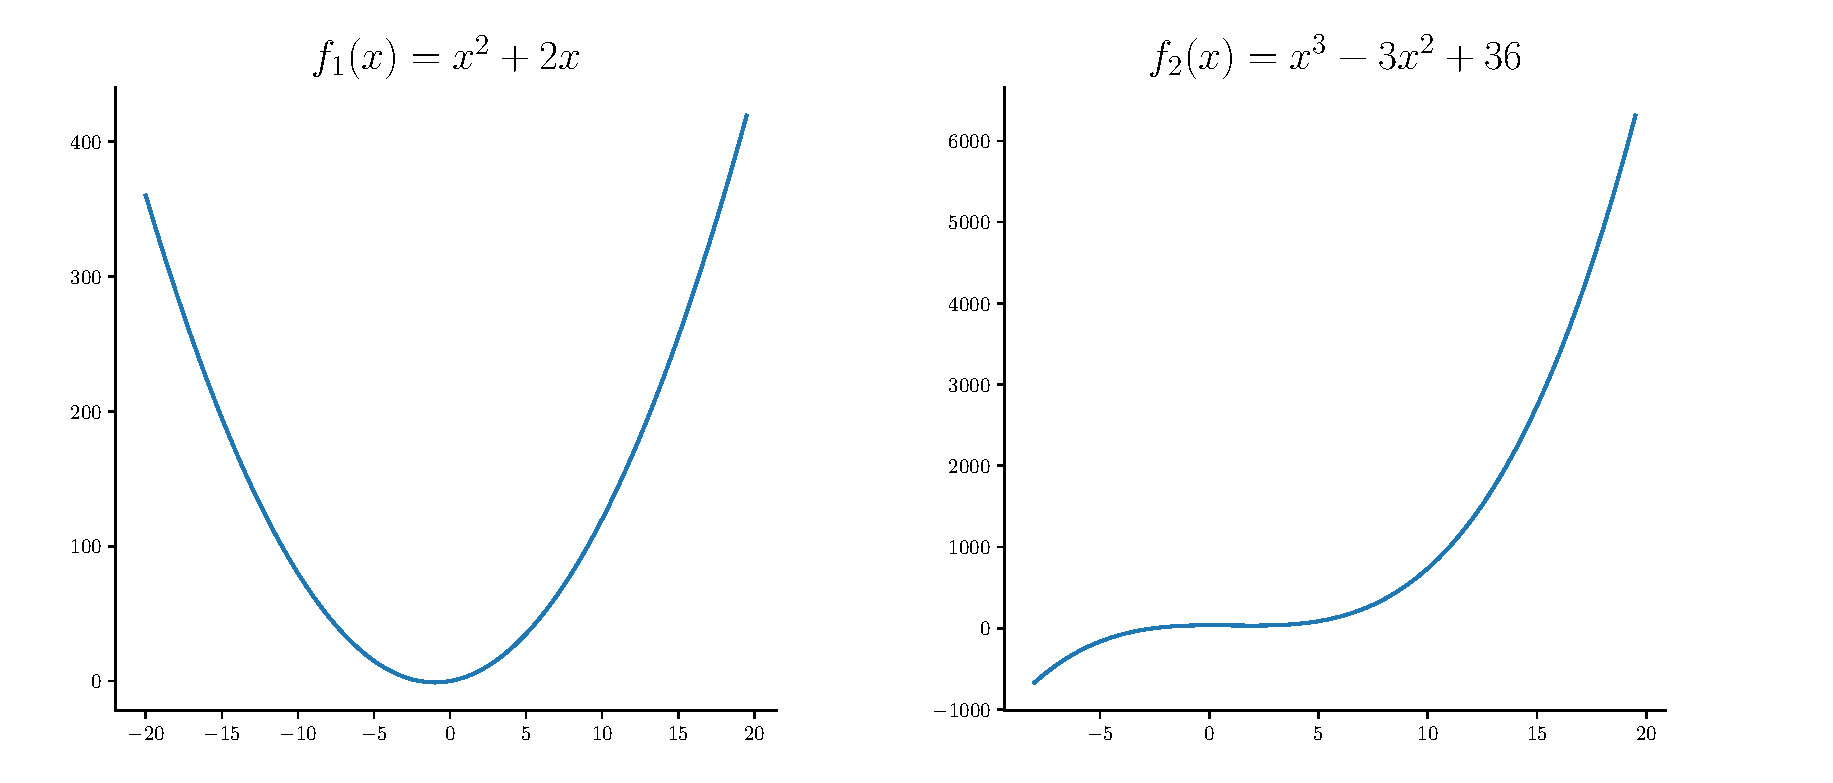
\includegraphics[width=\linewidth]{figs/functions.eps}
  \caption{Quadratic and non-quadratic functions for optmization.}
  \label{fig:functions}
\end{figure}

The estimated value for $x_{1}^*$ lies near $-1$, whereas the estimated value for $x_{2}^*$ lies near $8$. Hence, we can sample from a normal distribution for both functions:

\begin{align*}
X_1 &\sim \mathcal{N}(\mu_{1} = -1,\,\sigma_{1} = 1) \\
X_2 &\sim \mathcal{N}(\mu_{2} = 8,\,\sigma_{2} = 1)
\end{align*}

Furthermore, we will derive the number of iterations (stopping conditions) needed for the Fibonacci method to provide an accuracy of within $5\%$. We will define $I_0$ to be the initial interval, $I_n$ to be the final interval, and $F_n$ to be the $n^{th}$ Fibonnaci term.

Hence,

\begin{align*}
\frac{I_n}{2I_0} &\leq \frac{5}{100} \\
\frac{I_n}{I_0} &\leq \frac{1}{10} \\
\frac{1}{F_n} &\leq \frac{1}{10} \\
\end{align*}

Therefore,
$$F_n &\geq 10$$.

The value $n = 7$ was computed using Binet's formula for the Fibonacci terms. Fifteen random samples were then generated for both functions using the stopping criterion of $n = 7$ iterations. The table of results for both functions are shown in both Table 1 and Table 2.


\begin {table}[ht]
\centering
\caption {Results for $f_{1}(x) = x^2 + 2x$}
\begin{tabular}{lcccc}
\toprule
{} &    $x^*$ &     $f_{1}(x^*)$ &  function\_calls &  clock\_time \\
\midrule
  & -1.003858 & -0.999985 &            13.0 &    0.000258 \\
  & -0.999863 & -1.000000 &            12.0 &    0.000121 \\
  & -0.458484 & -0.706761 &            12.0 &    0.000142 \\
  & -0.133349 & -0.248917 &            12.0 &    0.000113 \\
  & -0.995906 & -0.999983 &            12.0 &    0.000107 \\
  & -1.794326 & -0.369046 &            12.0 &    0.000126 \\
  & -0.998712 & -0.999998 &            12.0 &    0.000121 \\
  & -0.675915 & -0.894969 &            12.0 &    0.000112 \\
  & -0.849852 & -0.977456 &            12.0 &    0.000097 \\
  & -0.998391 & -0.999997 &            12.0 &    0.000108 \\
  & -1.006449 & -0.999958 &            12.0 &    0.000099 \\
  & -1.009986 & -0.999900 &            12.0 &    0.000097 \\
  & -0.998913 & -0.999999 &            12.0 &    0.000097 \\
  & -1.293503 & -0.913856 &            12.0 &    0.000130 \\
  & -0.989732 & -0.999895 &            12.0 &    0.000165 \\
  & -0.493534 & -0.743493 &            12.0 &    0.000159 \\
  & -1.455641 & -0.792392 &            12.0 &    0.000164 \\
  & -0.779196 & -0.951246 &            12.0 &    0.000162 \\
  & -1.010637 & -0.999887 &            12.0 &    0.000120 \\
  & -0.995907 & -0.999983 &            12.0 &    0.000100 \\
\bottomrule
Avg: & -0.947108 & -0.879886 & 12.050 & 0.000158 \\
Std: & 0.351413 & 0.216419 & 0.224 & 0.000056 \\
\bottomrule
\end{tabular}
\end{table}


\begin {table}[ht]
\centering
\caption {Results for $f_{2}(x) = x^3 - 13x^2 + 36$}
\begin{tabular}{lcccc}
\toprule
{} &      $x^*$ &    $f_{2}(x^*)$ &  function\_calls &  clock\_time \\
\midrule
  &  7.699171 &  314.553840 &            13.0 &    0.000316 \\
  &  7.630426 &  305.599131 &            12.0 &    0.000154 \\
  &  7.940157 &  347.457533 &            12.0 &    0.000132 \\
  &  7.030768 &  235.247719 &            12.0 &    0.000120 \\
  &  7.778227 &  325.086647 &            12.0 &    0.000136 \\
  &  7.676198 &  311.540361 &            12.0 &    0.000131 \\
  &  7.471320 &  285.591838 &            12.0 &    0.000118 \\
  &  9.357814 &  592.745461 &            12.0 &    0.000137 \\
  &  7.949493 &  348.780494 &            12.0 &    0.000145 \\
  &  7.497876 &  288.862239 &            12.0 &    0.000126 \\
  &  7.477308 &  286.326859 &            12.0 &    0.000160 \\
  &  6.089015 &  150.528652 &            12.0 &    0.000166 \\
  &  8.458776 &  426.580208 &            12.0 &    0.000126 \\
  &  7.625984 &  305.026966 &            12.0 &    0.000138 \\
  &  8.655849 &  459.757240 &            12.0 &    0.000249 \\
  &  7.073400 &  239.804382 &            12.0 &    0.000280 \\
  &  7.573978 &  298.386878 &            12.0 &    0.000229 \\
  &  7.160760 &  249.349189 &            12.0 &    0.000226 \\
  &  7.293491 &  264.392311 &            12.0 &    0.000221 \\
  &  7.571402 &  298.060772 &            12.0 &    0.000213 \\
\bottomrule
Avg: & 7.650571 & 316.683936 & 12.050 & 0.000176 \\
Std:  & 0.664623 & 92.297258 & 0.224 & 0.000059\\
\bottomrule
\end{tabular}
\end {table}


\end{description}
\end{document}